\documentclass[aspectratio=169,11pt]{beamer}

% ============================================================
% PACKAGES
% ============================================================

\usepackage[T1]{fontenc}
\usepackage{lmodern}
\usepackage{amsmath,amssymb}
\usepackage{booktabs}
\usepackage{tikz}

\usetikzlibrary{positioning,arrows.meta}

% ============================================================
% BEAMER SETTINGS
% ============================================================

\setbeamertemplate{navigation symbols}{}

% ============================================================
% COLORS
% ============================================================

\definecolor{PaperWhite}{RGB}{248,250,252}
\definecolor{GridGray}{RGB}{215,222,230}
\definecolor{CyberBlue}{RGB}{35,95,160}
\definecolor{CyberCyan}{RGB}{0,145,170}
\definecolor{DarkText}{RGB}{35,45,55}
\definecolor{MutedText}{RGB}{100,110,120}
\definecolor{SoftBlue}{RGB}{235,243,250}
\definecolor{SoftCyan}{RGB}{235,249,250}

% ============================================================
% COLORS FOR BEAMER
% ============================================================

\setbeamercolor{normal text}{
	fg=DarkText,
	bg=PaperWhite
}

\setbeamercolor{structure}{
	fg=CyberBlue
}

\setbeamercolor{frametitle}{
	fg=CyberBlue,
	bg=PaperWhite
}

\setbeamercolor{title}{
	fg=CyberBlue
}

\setbeamercolor{subtitle}{
	fg=MutedText
}

% ============================================================
% BACKGROUND GRID
% ============================================================

\setbeamertemplate{background}
{
	
\begin{tikzpicture}[remember picture,overlay]
		
		% Background
		\fill[PaperWhite]
		(current page.south west)
		rectangle
		(current page.north east);
		
		% Small square grid
		\draw[
		GridGray,
		opacity=0.35,
		line width=0.25pt
		]
		(current page.south west)
		grid[
		step=0.5cm
		]
		(current page.north east);
		
		% Larger grid
		\draw[
		GridGray,
		opacity=0.18,
		line width=0.5pt
		]
		(current page.south west)
		grid[
		step=2.5cm
		]
		(current page.north east);
		
	\end{tikzpicture}
}

% ============================================================
% FRAME TITLE
% ============================================================

\setbeamertemplate{frametitle}
{
	\vspace{0.25cm}
	
	\begin{beamercolorbox}[wd=\paperwidth,
		leftskip=0.5cm,
		rightskip=0.5cm]
		{frametitle}
		
		\usebeamerfont{frametitle}
		\insertframetitle
		
	\end{beamercolorbox}
	
	
\begin{tikzpicture}
		
		\draw[
		CyberCyan,
		line width=1.2pt
		]
		(0,0) -- (11,0);
		
	\end{tikzpicture}
	
	\vspace{0.1cm}
}

% ============================================================
% FOOTER
% ============================================================

\setbeamertemplate{footline}
{
	\begin{tikzpicture}[remember picture,overlay]
		
		\draw[
		GridGray,
		line width=0.5pt
		]
		([yshift=0.35cm]current page.south west)
		--
		([yshift=0.35cm]current page.south east);
		
		\node[
		anchor=south west,
		font=\tiny,
		text=MutedText
		]
		at ([xshift=0.4cm,yshift=0.05cm]current page.south west)
		{
			Peter M. Ngugi | PhD Computer Science
		};
		
		\node[
		anchor=south east,
		font=\tiny,
		text=CyberBlue
		]
		at ([xshift=-0.4cm,yshift=0.05cm]current page.south east)
		{
			\insertframenumber
			/
			\inserttotalframenumber
		};
		
	\end{tikzpicture}
}

% ============================================================
% TITLE
% ============================================================

\title[
AI Cybercrime Forensics
]
{
	Forensics for Cybercrimes Committed Using Artificial Intelligence
}

\subtitle{
	A Digital Forensic Framework for AI-Assisted Cybercrime
}

\author{
	Peter M. Ngugi
}

\institute{
	PhD in Computer Science\\
	Zetech University
}

\date{
	2026
}

% ============================================================
% DOCUMENT
% ============================================================

\begin{document}
	
	% ============================================================
	% TITLE SLIDE
	% ============================================================
	
	\begin{frame}[plain]
		
		\begin{tikzpicture}[remember picture,overlay]
			
			% ==========================================================
			% 3D CUBE
			% ==========================================================
			
			% Front face
			\draw[
			CyberBlue,
			line width=1.4pt
			]
			(8,2)
			--
			(11,2)
			--
			(11,5)
			--
			(8,5)
			--
			cycle;
			
			% Top face
			\draw[
			CyberCyan,
			line width=1.4pt
			]
			(8,5)
			--
			(9.2,6.1)
			--
			(12.2,6.1)
			--
			(11,5);
			
			% Right face
			\draw[
			CyberBlue,
			line width=1.4pt
			]
			(11,2)
			--
			(12.2,3.1)
			--
			(12.2,6.1)
			--
			(11,5);
			
			% ==========================================================
			% CUBE NETWORK
			% ==========================================================
			
			\draw[
			CyberCyan,
			line width=1pt
			]
			(8.6,3)
			--
			(9.8,4)
			--
			(10.6,3.3);
			
			\fill[CyberCyan]
			(8.6,3) circle (3pt);
			
			\fill[CyberBlue]
			(9.8,4) circle (3pt);
			
			\fill[CyberCyan]
			(10.6,3.3) circle (3pt);
			
			% ==========================================================
			% EXTRA NODES
			% ==========================================================
			
			\fill[CyberCyan]
			(7.2,5.5) circle (2.5pt);
			
			\fill[CyberBlue]
			(13,4.8) circle (2.5pt);
			
			\draw[
			CyberCyan,
			opacity=0.5
			]
			(7.2,5.5) -- (9.8,4);
			
			\draw[
			CyberBlue,
			opacity=0.5
			]
			(10.6,3.3) -- (13,4.8);
			
		\end{tikzpicture}
		
		\vspace*{0.7cm}
		
		\begin{flushleft}
			
			{\fontsize{24}{28}\selectfont
				\bfseries
				\color{CyberBlue}
				Forensics for Cybercrimes
			}
			
			\vspace{0.1cm}
			
			{\fontsize{24}{28}\selectfont
				\bfseries
				\color{DarkText}
				Committed Using Artificial Intelligence
			}
			
			\vspace{0.35cm}
			
			{\color{CyberCyan}
				\rule{7cm}{2pt}
			}
			
			\vspace{0.4cm}
			
			{\large
				\color{MutedText}
				A Digital Forensic Framework for
				AI-Assisted Cybercrime
			}
			
			\vspace{0.8cm}
			
			{\large
				\color{DarkText}
				\textbf{Peter M. Ngugi}
			}
			
			\vspace{0.15cm}
			
			{\small
				\color{MutedText}
				PhD in Computer Science\\
				Zetech University
			}
			
			\vspace{0.15cm}
			
			{\small
				\color{MutedText}
				2026
			}
			
		\end{flushleft}
		
	\end{frame}
	
	% ============================================================
	% SLIDE 2
	% ============================================================
	
	\begin{frame}{Research Context}
		
		Artificial Intelligence is changing the cybercrime
		landscape.
		
		\vspace{0.4cm}
		
		\begin{columns}[T]
			
			\column{0.47\textwidth}
			
			\begin{block}{Traditional Cybercrime}
				
				\begin{itemize}
					
					\item Human-controlled systems
					
					\item Identifiable devices
					
					\item Conventional malware
					
					\item Established forensic procedures
					
				\end{itemize}
				
			\end{block}
			
			\column{0.47\textwidth}
			
			\begin{block}{AI-Assisted Cybercrime}
				
				\begin{itemize}
					
					\item Automated attacks
					
					\item Synthetic identities
					
					\item AI-generated content
					
					\item Autonomous decision-making
					
				\end{itemize}
				
			\end{block}
			
		\end{columns}
		
	\end{frame}
	
	% ============================================================
	% SLIDE 3
	% ============================================================
	
	\begin{frame}{The Forensic Challenge}
		
		\begin{center}
			
			
\begin{tikzpicture}[node distance=1.2cm]
				
				\node[
				draw=CyberCyan,
				fill=SoftCyan,
				rounded corners,
				minimum width=2.3cm,
				minimum height=0.9cm
				]
				(AI)
				{\textbf{AI}};
				
				\node[
				draw=CyberBlue,
				fill=SoftBlue,
				rounded corners,
				minimum width=2.3cm,
				minimum height=0.9cm,
				right=of AI
				]
				(C)
				{\textbf{Cybercrime}};
				
				\node[
				draw=CyberCyan,
				fill=SoftCyan,
				rounded corners,
				minimum width=2.3cm,
				minimum height=0.9cm,
				right=of C
				]
				(E)
				{\textbf{Evidence}};
				
				\node[
				draw=CyberBlue,
				fill=SoftBlue,
				rounded corners,
				minimum width=2.3cm,
				minimum height=0.9cm,
				right=of E
				]
				(F)
				{\textbf{Forensics}};
				
				\draw[
				->,
				>=Stealth,
				CyberCyan,
				line width=1pt
				]
				(AI) -- (C);
				
				\draw[
				->,
				>=Stealth,
				CyberCyan,
				line width=1pt
				]
				(C) -- (E);
				
				\draw[
				->,
				>=Stealth,
				CyberCyan,
				line width=1pt
				]
				(E) -- (F);
				
			\end{tikzpicture}
			
		\end{center}
		
		\vspace{0.7cm}
		
		\begin{center}
			
			\Large
			\textit{What happened?}
			
			\vspace{0.2cm}
			
			{\color{CyberCyan}$\Downarrow$}
			
			\vspace{0.2cm}
			
			\Large
			\textit{Who or what caused it?}
			
			\vspace{0.2cm}
			
			{\color{CyberCyan}$\Downarrow$}
			
			\vspace{0.2cm}
			
			\Large
			\textit{Can we prove it?}
			
		\end{center}
		
	\end{frame}
	
	% ============================================================
	% SLIDE 4
	% ============================================================
	
	\begin{frame}{Formalising Digital Evidence}
		
		Let
		
		\[
		E=\{e_1,e_2,\ldots,e_n\}
		\]
		
		represent the set of collected digital evidence.
		
		\vspace{0.3cm}
		
		Let
		
		\[
		A\subseteq E
		\]
		
		represent evidence that satisfies the authentication
		criteria.
		
		\vspace{0.3cm}
		
		Therefore:
		
		\[
		\boxed{A\subseteq E}
		\]
		
		\vspace{0.3cm}
		
		and
		
		\[
		e_i\in A
		\Rightarrow
		e_i\text{ satisfies the defined authentication criteria.}
		\]
		
	\end{frame}
	
	% ============================================================
	% SLIDE 5
	% ============================================================
	
	\begin{frame}{Forensic Evidence Pipeline}
		
		\begin{center}
			
			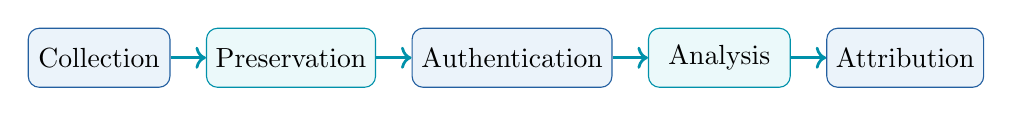
\begin{tikzpicture}[node distance=0.45cm]
				
				\node[
				draw=CyberBlue,
				fill=SoftBlue,
				rounded corners,
				minimum width=1.8cm,
				minimum height=0.75cm
				]
				(C)
				{Collection};
				
				\node[
				draw=CyberCyan,
				fill=SoftCyan,
				rounded corners,
				minimum width=1.8cm,
				minimum height=0.75cm,
				right=of C
				]
				(P)
				{Preservation};
				
				\node[
				draw=CyberBlue,
				fill=SoftBlue,
				rounded corners,
				minimum width=1.8cm,
				minimum height=0.75cm,
				right=of P
				]
				(A)
				{Authentication};
				
				\node[
				draw=CyberCyan,
				fill=SoftCyan,
				rounded corners,
				minimum width=1.8cm,
				minimum height=0.75cm,
				right=of A
				]
				(AN)
				{Analysis};
				
				\node[
				draw=CyberBlue,
				fill=SoftBlue,
				rounded corners,
				minimum width=1.8cm,
				minimum height=0.75cm,
				right=of AN
				]
				(AT)
				{Attribution};
				
				\draw[->,CyberCyan,line width=1pt] (C) -- (P);
				\draw[->,CyberCyan,line width=1pt] (P) -- (A);
				\draw[->,CyberCyan,line width=1pt] (A) -- (AN);
				\draw[->,CyberCyan,line width=1pt] (AN) -- (AT);
				
			\end{tikzpicture}
			
		\end{center}
		
		\vspace{0.6cm}
		
		\begin{block}{Core Principle}
			
			Evidence must remain traceable from collection through
			analysis and ultimately to attribution and presentation.
			
		\end{block}
		
	\end{frame}
	
	% ============================================================
	% SLIDE 6
	% ============================================================
	
	\begin{frame}{Research Objectives}
		
		\begin{block}{General Objective}
			
			To develop a digital forensic framework for investigating
			cybercrimes committed using Artificial Intelligence.
			
		\end{block}
		
		\vspace{0.3cm}
		
		\textbf{Specific Objectives}
		
		\begin{enumerate}
			
			\item Examine AI-assisted cybercrime techniques.
			
			\item Evaluate existing digital forensic approaches.
			
			\item Investigate evidence provenance and integrity.
			
			\item Develop a forensic framework.
			
			\item Evaluate the proposed framework.
			
		\end{enumerate}
		
	\end{frame}
	
	% ============================================================
	% SLIDE 7
	% ============================================================
	
	\begin{frame}{Expected Contribution}
		
		\begin{center}
			
			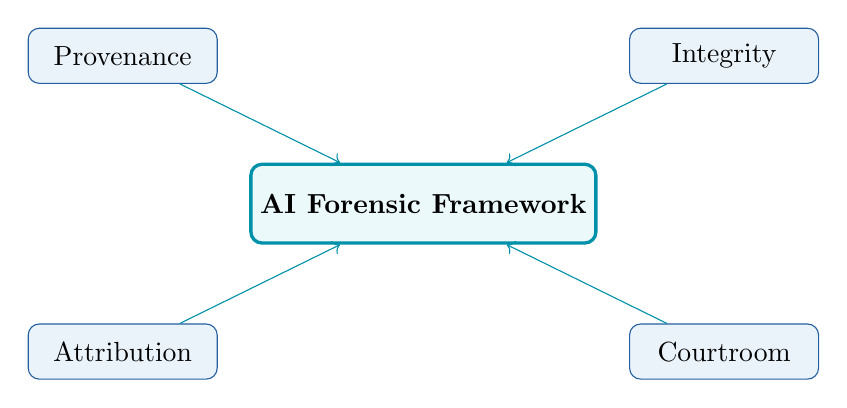
\begin{tikzpicture}
				
				\node[
				draw=CyberCyan,
				fill=SoftCyan,
				line width=1.2pt,
				rounded corners,
				minimum width=4cm,
				minimum height=1cm
				]
				(F)
				{\textbf{AI Forensic Framework}};
				
				\node[
				draw=CyberBlue,
				fill=SoftBlue,
				rounded corners,
				minimum width=2.4cm,
				minimum height=.7cm,
				above left=1cm and .4cm of F
				]
				(P)
				{Provenance};
				
				\node[
				draw=CyberBlue,
				fill=SoftBlue,
				rounded corners,
				minimum width=2.4cm,
				minimum height=.7cm,
				above right=1cm and .4cm of F
				]
				(I)
				{Integrity};
				
				\node[
				draw=CyberBlue,
				fill=SoftBlue,
				rounded corners,
				minimum width=2.4cm,
				minimum height=.7cm,
				below left=1cm and .4cm of F
				]
				(A)
				{Attribution};
				
				\node[
				draw=CyberBlue,
				fill=SoftBlue,
				rounded corners,
				minimum width=2.4cm,
				minimum height=.7cm,
				below right=1cm and .4cm of F
				]
				(C)
				{Courtroom};
				
				\draw[->,CyberCyan] (P) -- (F);
				\draw[->,CyberCyan] (I) -- (F);
				\draw[->,CyberCyan] (A) -- (F);
				\draw[->,CyberCyan] (C) -- (F);
				
			\end{tikzpicture}
			
		\end{center}
		
	\end{frame}
	
	% ============================================================
	% CONCLUSION
	% ============================================================
	
	\begin{frame}{Conclusion}
		
		\begin{block}{Central Argument}
			
			AI changes not only how cybercrimes can be committed,
			but also how digital evidence must be interpreted,
			authenticated and attributed.
			
		\end{block}
		
		\vspace{0.6cm}
		
		\begin{center}
			
			\[
			\boxed{
				\text{AI}
				+
				\text{Cybercrime}
				+
				\text{Digital Forensics}
				+
				\text{Evidence}
			}
			\]
			
		\end{center}
		
	\end{frame}
	
	% ============================================================
	% THANK YOU
	% ============================================================
	
	\begin{frame}[plain]
		
		\begin{center}
			
			\vspace{1.5cm}
			
			{\fontsize{34}{40}\selectfont
				\bfseries
				\color{CyberBlue}
				Thank You
			}
			
			\vspace{0.5cm}
			
			{\Large
				Questions \& Discussion
			}
			
			\vspace{1cm}
			
			{\large
				\textbf{Peter M. Ngugi}
			}
			
			\vspace{0.15cm}
			
			{\small
				PhD in Computer Science\\
				Zetech University
			}
			
		\end{center}
		
	\end{frame}
	
	% ============================================================
	
\end{document}